\documentclass[article, oneside]{oblivoir}
\usepackage{kotex}
\usepackage{graphicx}
\usepackage{mathtools}
\usepackage{hyperref} 
\usepackage{amsmath}
\usepackage{amssymb}
\usepackage{amsthm}
\hypersetup{colorlinks=false,}  
\usepackage{fapapersize}
\usefapapersize{210mm, 297mm,20mm,*,25mm,20mm}
\title{푸리에 해석과 미분방정식}
\author{esctabcapslock}
\makeindex
\begin{document}
\maketitle

\section{서론}
\subsection{목적과 개요}

\begin{itemize}
    \item 18세기 프링스의 수학자 조제프 푸리에 (Joseph Fourier, 1768 - 1830)가 열 전도 미방을  풀기 위해 만듦
    \item 어떤 함수가 있으면, 그 함수를 삼각함수의 합으로 표현한다. 기저를 바꾼다.
    \item 전자, 전기, 통신, 기계, 구조공학, 소리 등 아주 다양한 공학 분야에서 활용 중
    \item 이를 이용하면 불확정성 원리 증명할 수 있음.
    \item 이를 응용하면 다음과 같은 이퀄라이저를 만들 수 있다. 다음 주소(링크) 참조: \href{https://esctabcapslock.github.io/WebAudioAPI/푸리에.html}{푸리에.html}\footnote{\href{https://esctabcapslock.github.io/WebAudioAPI/푸리에.html}{https://esctabcapslock.github.io/WebAudioAPI/푸리에.html}, 본인 github임}
    \item 푸리에 변환 $\cup$ 푸리에 급수 $=$ 푸리에 해석임.
\end{itemize}
어떤 함수가 있다. 시간에 따라 변하는 함수라고 하자. 이 함수를 요리하고 싶은데, 뭔가 어렵고 막막하다.

\begin{figure}[ht]
    \centering
    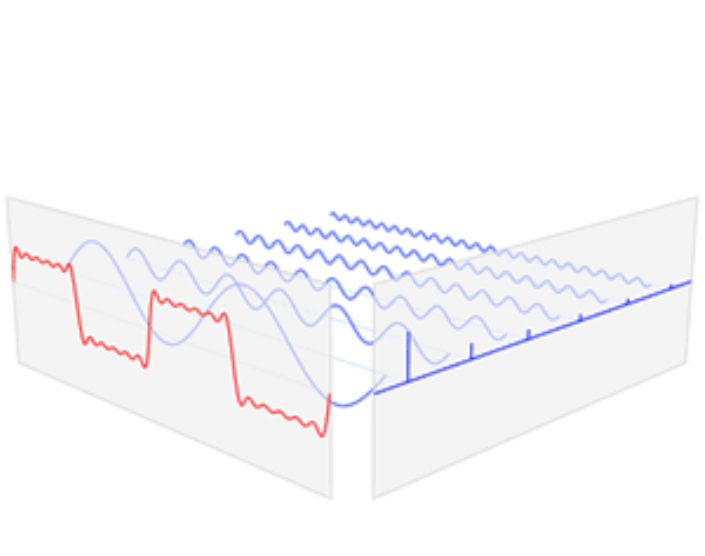
\includegraphics[width=.4\textwidth]{./img/3.png}
    \caption{시간에 대한 값들의 모임에서, 주기와 진폭의 모임들로 바꿔서 생각한다. 출처: \href{https://en.wikipedia.org/wiki/File:Fourier_transform_time_and_frequency_domains_(small).gif}{위키미디어 공용}}
    \label{fig:my_label}
\end{figure}
%https:\/\/javalab.org\/fourier_analysis 

\subsection{수학적 연관성}

우리는, 작년에 적률생성함수에 대해 배웠다. 말 그대로, 특정 확률 분포의 적률을 생성하는 함수이다. 확률변수 $X$에 대해, 확률밀도함수가 $f(x)$일때, 적률생성함수 $M_X(t)$는 다음과 같았다. 우리는 이를 이용해 $E(X^n)$을 기계적으로 구할 수 있었다.

\begin{equation}
    M_X(t) = E[e^{tx}] = \int_{-\infty}^{\infty} e^{tx} f(x) dx
\end{equation}

적률생성함수가 같으면, 같은 확률밀도함수다.

사실, 이는 라플라스 변환의 일종이다. 라플라스 변환은 다음과 같이 정의된다. 푸리에 변환과 성질이 아주 비슷하며, 여러 재미있는 수학적 성질들이 있다.


\begin{equation}
    F(s) = \mathcal{L}\left\{f\right\}(s) = \int_0^{\infty}e^{-st} f(t) dt
\end{equation}

사실, 이것은 푸리에 변환과 아주 비슷하다. 푸리에 변환은 다음과 같이 정의된다. (정의나, 계수는 책마다 다르다) 익스퍼넨셜 함수 지수 부분을, 복소수를 약간 치환한 형태다. 

\begin{equation}
    X(s) = \mathcal{F}\left\{x\right\}(s) = \int_{-\infty}^{\infty}e^{-2 \pi i s t} x(t) dt
\end{equation}



%\mu_n = \int_{-\infty}^{\infty} (x-c)^n P(x=X) dx
\section{실수에서 푸리에 급수}
구간 $2L$의 주기를 갖고, $\mathbb{R}$로 가며, 부분적으로 연속인 (=적분 가능한) 함수들의 집합 $F$을 생각하자.

$$B = \left\{1, \sin \left(\frac{\pi x}{L}\right), \quad \cos \left(\frac{\pi x}{L}\right), \sin \left(\frac{2 \pi x}{L}\right),  \cos \left(\frac{2 \pi x}{L}\right) \cdots, \right\}$$

는 $F$의 직교족이다.\footnote{2021 1학기 선형대수 참조} \footnote{내적의 정의 $\left\langle f\mid g\right\rangle = \int f(x) g(g) dx $ 에 의해 서로 다른 내적하면 0이며, 같은 것끼리 내적하면 $L$임}


그리고, 이 기저 후보들로 사영시킨 것들을 다시 더함으로써 다시 $F$의 모든 원소를 생성할 수 있다. 따라서, $B$는 기저다. 다음의 급수를 푸리에 급수라 한다. 적분 가능한 함수라면, 푸리에 급수는 $f(x)$로 수렴한다. $\epsilon-\delta$로 증명 가능하며, 증명은 생략한다.

\begin{equation}
    f(t) = \lim_{N \to \infty} S_N^f (t) = \frac{1}{2} a_0 + \sum_{n=1}^{\infty} \left( a_n \cos \frac{n \pi t}{L} + b_n sin \frac{n \pi t}{L}\right)
\end{equation}
그리고, 각 계수들은 당연하게도
$a_0 = \frac{1}{L} \int_{-L}^{L} f(t)dt
= \frac{1}{L} \left\langle f(t) \mid 1\right\rangle$$
, a_n = \frac{1}{L} \int_{-L}^{L} f(t) \cos\frac{n \pi t}{L}dt 
=\frac{1}{L} \left\langle f(t) \mid \cos\frac{n \pi t}{L}\right\rangle, b_n = \cdots$ 이렇게 각 기저 성분을 모은 것으로 표현할 수 있다.

\section{복소수에서의 푸리에 급수}
$c_n = \frac{1}{2}\left(a_n - ib_n\right)$, $c_{-n} = \frac{1}{2}\left(a_n + ib_n\right)$으로 정의한다면, $c_n = \frac{1}{2L}\int_{-L}^{L} f(t)e^{i\frac{n \pi t}{L}}$이 나온다. 간단하게 정리하면\footnote{$\cos \theta = \frac{e^{i \theta} + e^{-i \theta}}{2}$ 등 오일러 공식 활용}, 본 급수는 더 깔끔하게, 다음과 같이 쓸 수 있다.
\begin{equation}
    f(t) = \sum_{n=-\infty}^{\infty} c_n e^{i \frac{n \pi t}{L}}
\end{equation}

%https://freshrimpsushi.github.io/posts/complex-representation-of-fourier-series/
\section{푸리에 변환과 역변환}

주가함수가 아니라, 일반적 함수에 대해 적용시키면 푸리에 변환이다. $\lim_{x \to \pm \infty}f(x)=0$이고 적분 가능한 일반적인 $f$에서, 유도해 보자.
$\Delta \xi = \frac{\pi}{L}$, $F(n) = \int_{-L}^{L} f(t)e^{i\frac{n \pi t}{L}}$으로 두면 다음이 성립한다. 
$$f(t) = \frac{L}{\pi} \sum_{n=-\infty}^{\infty} c_n e^{i \Delta \xi n t} = \frac{1}{2\pi} \sum_{n=-\infty}^{\infty} F(n) e^{i  \Delta \xi n t} \Delta \xi$$
그리고 $L \to \infty$로 두면, $\Delta \xi \to 0$이다. 위 식은 리만합으로써 적분꼴로 쓸 수 있다.

\begin{equation}
    f(t) = \frac{1}{2\pi} \int_{-\infty}^{\infty} F(n) e^{i \xi t}d\xi \quad F(\xi) = \int_{-\infty}^{\infty} f(t)e^{-i \xi t}dt
\end{equation}

$F$는 $f$의 푸리에 변환이며, 반대 과정을 푸리에 역변환이라고 한다. $F(\xi)$는 $\mathcal{F}\left\{f\right\}(\xi)$로 쓴다.\footnote{정의는 책마다 조금씩 다르다.} 변환 후, 역변환하면 자기 자신이므로, $\mathcal{F}\{f\} = \mathcal{F}\{g\}$면 $f=g$가 성립한다.
또한, 선형성도 갖고 있어, 임의의 상수 $a$, $b$에 대해 $\mathcal{F} \left[af(x)+bg(x)\right]=a\mathcal{F} \left[f(x)\right]+b\mathcal{F} \left[g(x)\right]$도 만족한다.

%\section{응용: 불확정성 원리}
%https://freshrimpsushi.github.io/posts/various-meanings-of-fourier-transforms/
%https://freshrimpsushi.github.io/posts/properties-of-fourier-transform/
\section{응용: 1차원 열전도 미분방정식의 풀이}
푸리에 급수를 이용해서도 미방을 풀 수 있으나, 생략하겠다.

푸리에 변환의 정의에서, 부분적분을 하면 다음을 보일 수 있다.
\begin{equation}
    \mathcal{F}\left\{f' \right\} (\xi) = i \xi \mathcal{F}\left\{f \right\} (\xi), \quad \mathcal{F}\left\{f^n \right\} (\xi) = \left(i \xi\right)^n \mathcal{F}\left\{f \right\} (\xi), \label{eq:b2}
\end{equation}
여기서, 변환표를 이용하면 선형 미방의 해를 쉽게 답을 구할 수 있다.
\footnote{라플라스 변환도 이런 식이 존재한다. 다만 약간 복잡하다. 이건 실수에서만 생각하기 때문!}
일차원 열 미분방정식을 풀어보자.
$\mathcal{F}\{u\}(\xi, t) = U(\xi, t)$, $\mathcal{F}\{f\}(x) = F(\xi)$로 정의한다.

$$\frac{\partial u(x,t)}{\partial t} = \frac{\partial^2 u(x,t)}{\partial x^2}, \quad (-\infty < x < \infty), \quad f(x) = u(x,0) $$

양변에 푸리에 변환을 취하고, \ref{eq:b2}번 식을 적용하자.
$$\mathcal{F}\{u_t\}(\xi, t) = k \mathcal{F}\{u_{xx}\}(\xi, t) =  - k \xi^2 \mathcal{F}\{u\}(\xi, t)$$

또한, 함수의 성질이 좋아서 적분과 미분을 바꿀 수 있다 하자. 그렇다면 $\mathcal{F}\{u_t\} = \frac{\partial}{\partial t}\mathcal{F}\{u\}$이 성립한다. 그러면 주어진 식은 간단한 선형 상미분 방정식이 된다.

$$\frac{\partial U(\xi, t)}{\partial t} = - k \xi^2 U(\xi, t)$$

풀면, $U(\xi, t) = F(\xi) e^{-k \xi ^2 t}$이다. 여기에서 양변을 각각 푸리에 역변환해 주면, $u(x,t)$에 대한 식이 나오므로, 우리가 원하는 해답이 된다.

$$u(x,t) = \frac{1}{\sqrt{4 \pi k t}} \int f(y) e^{-\frac{\left(x-y\right)^2}{4 k t}} dy$$

\section{참고문헌}
\begin{itemize}
    \item \href{https://freshrimpsushi.github.io/}{블로그: 생새우초밥집 \> 푸리에 해석 카테고리} \footnote{https://freshrimpsushi.github.io}
    \item 도서: (핵심) Fourier 해석과 복소해석 Fourier analysis \& complex analysis, 전병재 지음, 텍스트북스
\end{itemize}
\end{document}
